\documentclass[journal,10pt,twocolumn]{article}
\usepackage{graphicx}
\usepackage[margin=0.5in]{geometry}
\usepackage[cmex10]{amsmath}
\usepackage{array}
\usepackage{booktabs}
\usepackage{mathtools}
\title{\textbf{Optimization Assignment - 2}}
\author{Akana Sai Kumar}


\providecommand{\norm}[1]{\left\lVert#1\right\rVert}
\providecommand{\abs}[1]{\left\vert#1\right\vert}
\let\vec\mathbf
\newcommand{\myvec}[1]{\ensuremath{\begin{pmatrix}#1\end{pmatrix}}}
\newcommand{\mydet}[1]{\ensuremath{\begin{vmatrix}#1\end{vmatrix}}}
\providecommand{\brak}[1]{\ensuremath{\left(#1\right)}}
\providecommand{\lbrak}[1]{\ensuremath{\left(#1\right.}}
\providecommand{\rbrak}[1]{\ensuremath{\left.#1\right)}}
\providecommand{\sbrak}[1]{\ensuremath{{}\left[#1\right]}}

\begin{document}

\maketitle
\paragraph{\textit{Problem Statement} -Show that the altitude of the right circular cone of maximum volume that can be inscribed in a sphere of radius R is 4R/3}
\section*{\large Solution}
Let $r$=5\\
volume of cone is given 
 V = $\frac{1}{3}$$\pi$$R^2$h\\
 h=r+$\sqrt{r^2-R^2}$  
 \begin{align}
V=\frac{1}{3} \pi R^2r+\frac{1}{3}\pi R^2\sqrt{r^2-R^2}\\
V'=\frac{2}{3}\pi Rr+\frac{2\pi R r^2-3\pi R^3}{3\sqrt{r^2-R^2}}
\end{align}
 



\subsection*{\normalsize Gradient descent}

\begin{align}
	\label{eq:vol_varx}
	\implies V = \frac{1}{3} \pi R^2r+\frac{1}{3}\pi R^2\sqrt{r^2-R^2}
\end{align}

    \begin{align}
        x_{n+1} &= x_n + \alpha \nabla V \\
        \implies x_{n+1} &= x_n + \alpha \brak{\frac{2}{3}\pi Rr+\frac{2\pi R r^2-3\pi R^3}{3\sqrt{r^2-R^2}}}
    \end{align}
    
Taking $x_0=r-1,\alpha=0.001$ and precision = 0.00000001, values obtained using python are:
    
    \begin{align}
        \boxed{\text{Maxima} = 155.14037795505135}\\
        \boxed{\text{Maxima Point} = 4.71404516335876}
    \end{align}

Ploting
\centering{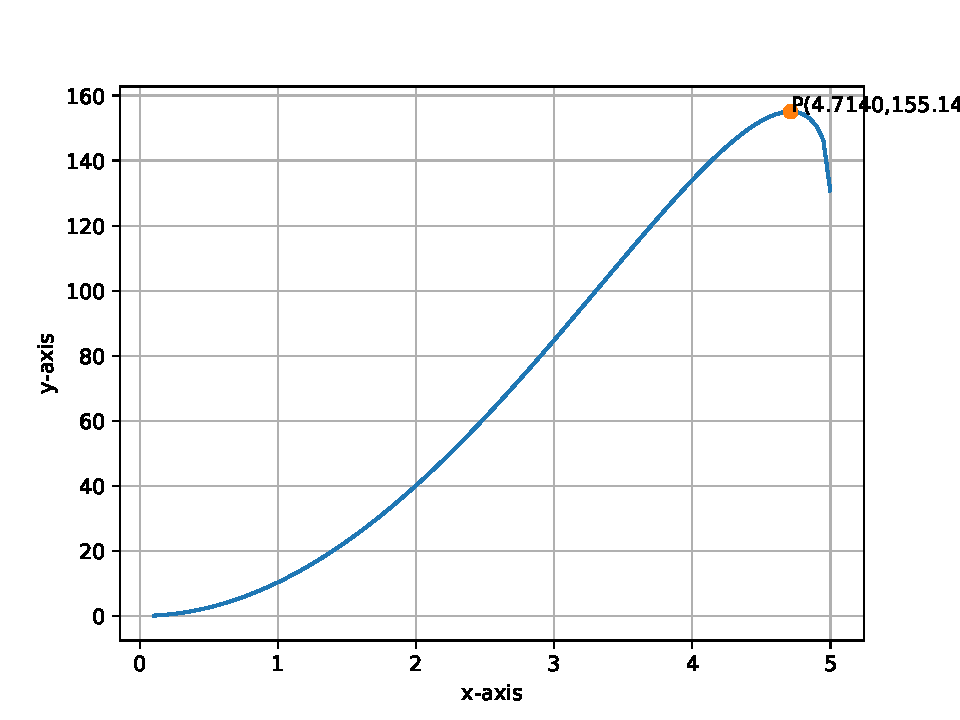
\includegraphics[scale=0.5]{opt0.pdf}}



\begin{figure}[t]
	\centering
%	\includegraphics[width=1\columnwidth]{opt.pdf}
%	\caption{Graph of $S(l)$ vs $l$}
%	\label{fig:graph_fx}
\end{figure}

\end{document}